\documentclass{article}

\usepackage{tikz}
\usetikzlibrary{calc, positioning, shapes.geometric}
\usepackage[dvipsnames]{xcolor}

\usepackage{Sweave}
\begin{document}
\Sconcordance{concordance:jogo-extensivo2.tex:jogo-extensivo2.Rnw:1 34 1}

\Sconcordance{concordance:jogo-bofsex-nature1.tex:jogo-bofsex-nature1.Rnw:1 6 1 1 0 %
82 1}


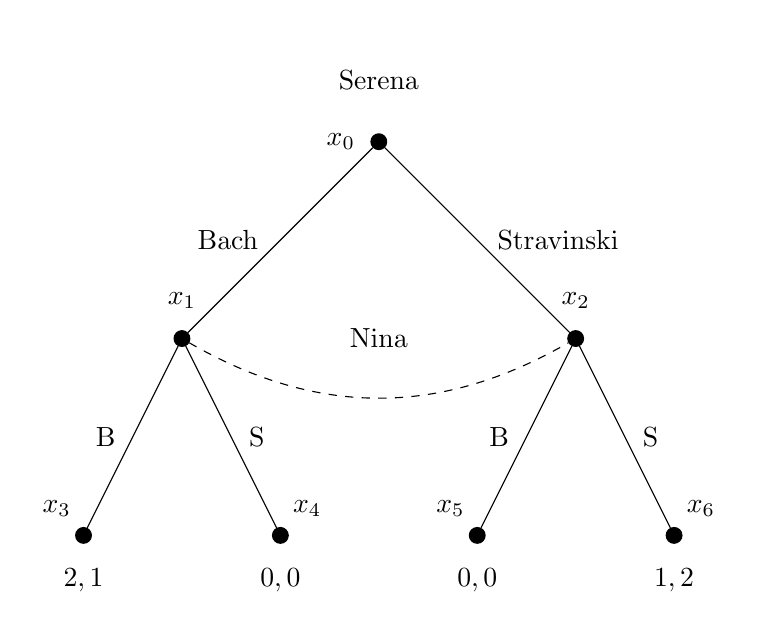
\begin{tikzpicture}[>=stealth, every node/.style={circle}]
\tikzstyle{solid node}=[draw, circle, fill=black, inner sep=1.5, minimum size=2mm]
\tikzstyle{decision}=[draw, rectangle, fill=gray!30]
\tikzstyle{level 1}=[sibling distance=50mm, level distance=25mm]
\tikzstyle{level 2}=[sibling distance=25mm, level distance=25mm]


\node[solid node, label=above:{Serena}, label=left:{$x_0$}] (serena) {}
  child{node[solid node, label=above:{}, label=above:{$x_1$}] (nina1){}
    child{node[solid node,label=below:{$2,1$}, label=above left:{$x_3$}]{} edge from parent node[left]{B}}
    child{node[solid node,label=below:{$0,0$}, label=above right:{$x_4$}]{} edge from parent node[right]{S}}
  edge from parent node[left,xshift=-3]{Bach}
  }
  child{node[solid node, label=above:{}, label=above:{$x_2$}] (nina2) {}
    child{node[solid node,label=below:{$0,0$}, label=above left:{$x_5$}]{} edge from parent node[left]{B}}
    child{node[solid node,label=below:{$1,2$}, label=above right:{$x_6$}]{} edge from parent node[right]{S}}
  edge from parent node[right,xshift=3]{Stravinski}
  };

\node at ($(nina1)!.5!(nina2)$) {Nina};
\draw[dashed,bend right](nina1)to(nina2);
\end{tikzpicture}

\end{document}
